% Created 2020-11-03 Tue 10:26
% Intended LaTeX compiler: pdflatex
\documentclass[presentation, aspectratio=169]{beamer}
\usepackage[utf8]{inputenc}
\usepackage[T1]{fontenc}
\usepackage{graphicx}
\usepackage{grffile}
\usepackage{longtable}
\usepackage{wrapfig}
\usepackage{rotating}
\usepackage[normalem]{ulem}
\usepackage{amsmath}
\usepackage{textcomp}
\usepackage{amssymb}
\usepackage{capt-of}
\usepackage{hyperref}
\RequirePackage{fancyvrb}
\usepackage[margin=0.5in]{geometry}
\usepackage[backend=bibtex]{biblatex}
\addbibresource{./../biblio.bib}
\author[A. Caliò]{Antonio Caliò\inst{1}}
\usetheme{default}
\date{}
\title{The Spark Ecosystem}
\institute{\inst{1}DIMES Dept., University of Calabria\\ Rende (CS), IT \\ a.calio@unical.it\\ Big Data Analytics - Computer Engineering for the IoT}
\titlegraphic{\begin{picture}(0,0) \put(200,200){\makebox(0,0)[rt]{
\includegraphics[width=3cm]{./img/logo_dimes.jpg}}} \end{picture}}}
\AtBeginSection[]{\begin{frame}<beamer>\frametitle{Presentation agenda}\tableofcontents[currentsection]\end{frame}}
\hypersetup{
 pdfauthor={},
 pdftitle={The Spark Ecosystem},
 pdfkeywords={},
 pdfsubject={},
 pdfcreator={Emacs 27.1 (Org mode 9.3)}, 
 pdflang={English}}
\begin{document}

\maketitle
\begin{frame}{Outline}
\tableofcontents
\end{frame}





\section{Introduction}
\label{sec:orgdf77702}

\begin{frame}[label={sec:orga3f0b8c}]{What is Spark}
\begin{itemize}
\item Apache SparkTM is a fast and general-purpose engine for large-scale data processing
\item Spark is designed to achieve the following goals:
\begin{itemize}
\item Generality: diverse workloads, operators, job sizes
\item Low latency: sub-second
\item Fault tolerance: faults are the norm, not the exception
\item Simplicity: often comes from generality
\end{itemize}
\end{itemize}
\end{frame}

\begin{frame}[label={sec:org67f0000}]{Motivation}
\begin{itemize}
\item Spark's main goal is to overcome one major limitation of the Map-Reduce approach: 
\begin{itemize}
\item The need for a lot of I/O operation.
\end{itemize}
\end{itemize}

\begin{figure}[htbp]
\centering
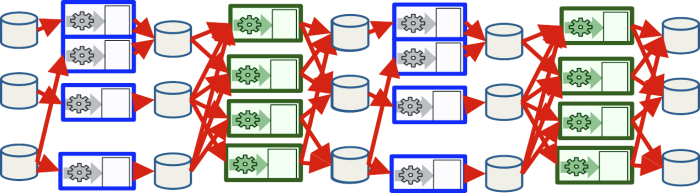
\includegraphics[width=.9\linewidth]{./img/map-reduce.png}
\caption{\label{fig:org4caa872}Map-Reduce}
\end{figure}

\pause
\begin{itemize}
\item \alert{Solution}: Keep data in main memory
\end{itemize}
\end{frame}



\begin{frame}[label={sec:org171b951},t]{MapReduce vs Spark}
\begin{column}{0.5\columnwidth}
\begin{itemize}
\item Iterative jobs
 \begin{figure}[htbp]
\centering
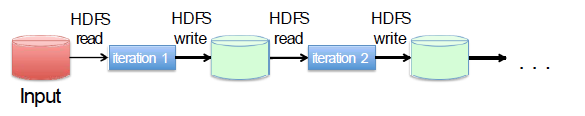
\includegraphics[width=.9\linewidth]{./img/mr-iterative.png}
\caption{\label{fig:orgbbc37f3}M/R}
\end{figure}
n\#+caption: Spark 
\begin{center}
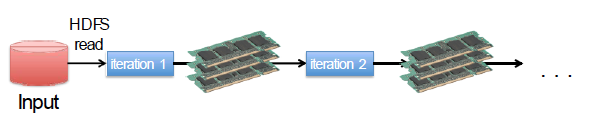
\includegraphics[width=.9\linewidth]{./img/spark-iterative.png}
\label{orgef90637}
\end{center}
\end{itemize}
\end{column}

\begin{column}{0.5\columnwidth}
\begin{itemize}
\item Same data multiple jobs
\begin{figure}[htbp]
\centering
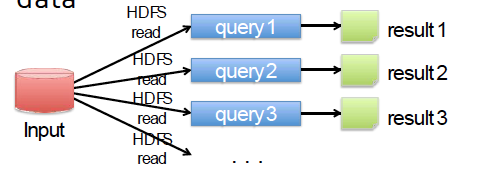
\includegraphics[width=.9\linewidth]{./img/map-multiple.png}
\caption{\label{fig:orgca23053}M/R}
\end{figure}
\end{itemize}
\begin{figure}[htbp]
\centering
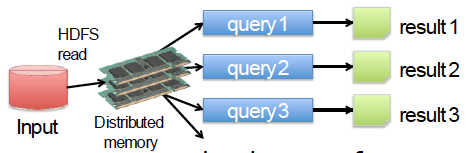
\includegraphics[width=.9\linewidth]{./img/spark-multiple.png}
\caption{\label{fig:org9b5503f}Spark}
\end{figure}
\end{column}
\end{frame}

\section{Spark Key Concepts}
\label{sec:org9dd9540}

\begin{frame}[label={sec:org1e1db8c}]{Spark Components}
\begin{figure}[htbp]
\centering
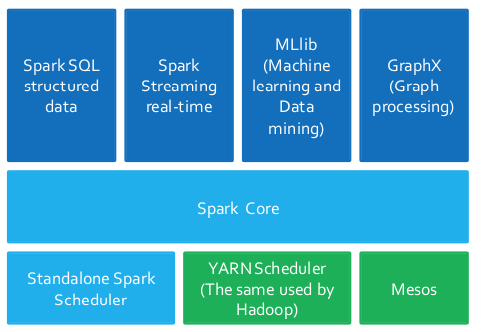
\includegraphics[width=9cm,height=7cm]{./img/spark-eco.png}
\caption{\label{fig:org6a3b0d3}Spark overview}
\end{figure}
\end{frame}

\begin{frame}[label={sec:org9b2860b}]{Spark Core}
\begin{itemize}
\item It is the main building block  that is exploited by all the high-level data analytics components
\item It contains the basic functionalities of Spark exploited by all components
\begin{itemize}
\item Task scheduling
\item Memory management
\item Fault recovery
\end{itemize}

\item Provides the APIs that are used to create RDDs and applies transformations and actions upon them
\end{itemize}
\end{frame}


\begin{frame}[label={sec:orgd2636ea}]{Cluster Mode}
\begin{figure}[htbp]
\centering
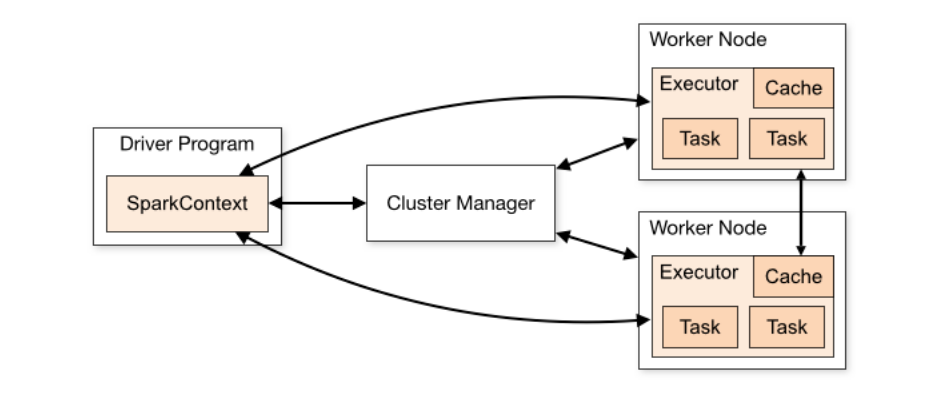
\includegraphics[width=9cm,height=4cm]{./img/cluster-mode.png}
\caption{\label{fig:org9a7a3cd}Cluster mode}
\end{figure}

\begin{itemize}
\item There are four possible options for the cluster manager:
\begin{itemize}
\item Standalone (included in spark and used by default)
\item Apache Mesos
\item Hadoop YARN
\item Kubernets
\end{itemize}
\end{itemize}
\end{frame}

\begin{frame}[label={sec:org379d093}]{Resilient Distributed Datasets (RDDs)}
\begin{itemize}
\item Partitioned/Distributed collections of objects spread across the nodes of a clusters
\item Stored in main memory (when it is possible) or on local disk
\item Spark programs are written in terms of operations on resilient distributed data sets

\item RDDs are built and manipulated through a set of parallel:
\begin{itemize}
\item Transformations  (e.g., map, filter, join)
\item Actions  (e.g., count, collect, save)
\item RDDs are automatically rebuilt on machine failure
\end{itemize}

\item They are split in partitions
\begin{itemize}
\item Each node of the cluster that is running an application is assigned with at least one
partition of some RDD
\end{itemize}
\item RDDs are can be stored:
\begin{itemize}
\item In  the main memory of the executor node
\item In the local disk of the executor node
\end{itemize}
\item RDD enables parallel and distributed computation on the node-level
\end{itemize}
\end{frame}


\begin{frame}[label={sec:orgf78c1a8}]{Example}
\begin{figure}[htbp]
\centering
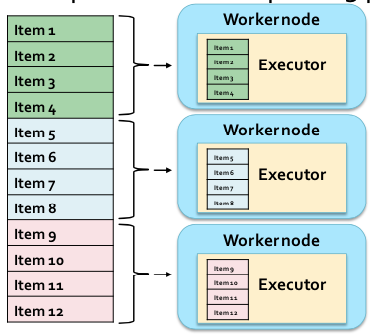
\includegraphics[width=7cm,height=6cm]{./img/rdd-examplepng.png}
\caption{\label{fig:org3ff1346}RDDs partition. Having more partitions implies having more parallelsm}
\end{figure}
\end{frame}


\begin{frame}[label={sec:org61cb394}]{RDDs Properties}
\begin{itemize}
\item An RDD is \emph{immutable}, i.e., its content cannot be modified
\item An RDD can be created starting from:
\begin{itemize}
\item a parallelized collection of objects
\item any file stored in a HDFS or in a regular file system
\item a database
\item another existing RDD
\end{itemize}
\end{itemize}
\end{frame}


\begin{frame}[label={sec:org761806d}]{Spark program}
\begin{itemize}
\item Spark programs are written in terms of operations on RDDs
\begin{itemize}
\item Transformations
\item Actions
\end{itemize}

\item Spark programs are responsible for:
\begin{itemize}
\item Scheduling and synchronization of the jobs
\item Splitting of RDDs in partitions and allocation RDDs’ partitions in the nodes of the cluster
\item Hiding complexities of fault-tolerance and slow machines
\end{itemize}

\item Spark programs can be written in a variety of languages: Java, Python, Scala, R
\end{itemize}
\end{frame}

\begin{frame}[label={sec:orgdb1b7e4}]{The driver program}
\begin{columns}
\begin{column}{0.5\columnwidth}
\begin{itemize}
\item It is basically the file containing the main method
\item It defines the workflow of the application
\item It defines the necessary RDDs
\item It accesses the spark cluster through a \emph{SparkContext} object
\begin{itemize}
\item The driver program actually runs on the executors involved in the cluster
\item Each executor runs on its partition of the RDD
\end{itemize}
\end{itemize}
\end{column}
\begin{column}{0.5\columnwidth}
\begin{figure}[htbp]
\centering
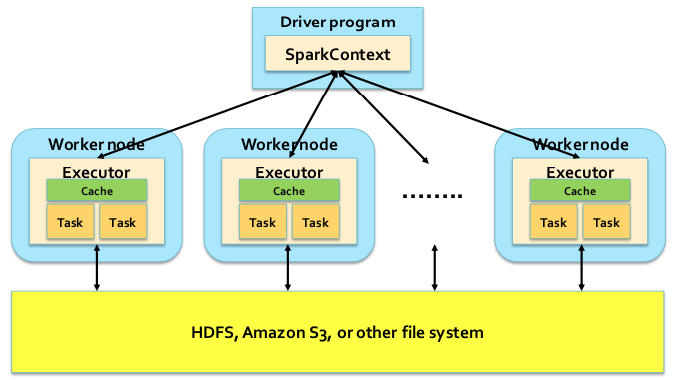
\includegraphics[width=.9\linewidth]{./img/driver-program.png}
\caption{\label{fig:org4febdf8}Driver program}
\end{figure}
\end{column}
\end{columns}
\end{frame}
\section{RDDs Main Operations}
\label{sec:orgdbdd776}
\begin{frame}[label={sec:org439c241},fragile]{Creation}
 \begin{itemize}
\item From a text file
\begin{verbatim}
val logData = spark.read.textFile(logFile)
\end{verbatim}
\end{itemize}
\begin{itemize}
\item From a collection
\begin{verbatim}
spark.sparkContext.parallelize(<somelist>)    
\end{verbatim}
\end{itemize}
\begin{itemize}
\item From another RDD
\begin{verbatim}
val nextRdd = rdd.<someRDDTransformation>((x, y) => x+y)
\end{verbatim}
\end{itemize}
\end{frame}
\begin{frame}[label={sec:orgefd4038},fragile]{Storage}
 \begin{itemize}
\item Calling the cache function
\end{itemize}
\begin{verbatim}
val logData = spark.read.textFile(logFile).cache()
\end{verbatim}
This function actually calls: \texttt{persist(SotrageLevel.MEMORY\_AND\_DISK)}



\begin{columns}
\begin{column}{0.5\columnwidth}
\begin{itemize}
\item \alert{Why caching?} - If your spark program defines a similar DAG as the one in ..
Then it makes sense to save the RDD generated after step 2 as it will feed 
two distinct branches of your application
\item More generally, you should cache any RDD that will be used more than once
\end{itemize}
\end{column}

\begin{column}{0.5\columnwidth}
\begin{center}
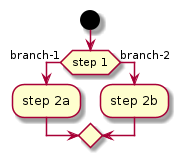
\includegraphics[width=.9\linewidth]{dag.png}
\end{center}
\end{column}
\end{columns}
\end{frame}

\begin{frame}[label={sec:org1dee3da}]{StorageLevel}
\begin{itemize}
\item There are four different storage levels:
\begin{itemize}
\item DISK\_ONLY: Persist data on disk only in serialized format
\item MEMORY\_ONLY:  Persist data in memory only in deserialized format
\item MEMORY\_AND\_DISK: Persist data in memory and if enough memory is not available evicted blocks will be stored on disk
\item OFF\_HEAP: Data is persisted in off-heap memory
\end{itemize}
\end{itemize}
\end{frame}

\begin{frame}[label={sec:org23612f8},fragile]{Retrieval}
 \begin{itemize}
\item The content of an RDD can be retrieved from the nodes of the cluster and “stored” in a local  variable
of the Driver process.
\end{itemize}
\begin{verbatim}
val collectedVariable: Array[<RDD objects'type>] = RddVariable.collect()
\end{verbatim}
\begin{itemize}
\item The \texttt{collect()} method returns all the elements in the RDD as a collection of objects
\begin{itemize}
\item Be aware that if the size of the RDD is to large it may not fit inside a regular (not-distributed) variable
\end{itemize}
\end{itemize}
\end{frame}


\begin{frame}[label={sec:org9cbe302}]{Transformations}
\begin{itemize}
\item Operations on RDDs that return a new RDD
\item Apply a transformation on the elements of the input RDD(s) and the result of the transformation is stored in a new RDD
\begin{itemize}
\item Remember that RDDs are immutable, i.e., we cannot change the content of an already existing RDD
\item We can only apply a transformation on the content of an RDD and store/assign the result in/to a new RDD
\end{itemize}
\item Transformations  are computed lazily 
\begin{itemize}
\item i.e., transformations are computed only when an action is applied on the RDDs generated by the transformation operations
\item When a transformation is invoked Spark keeps only track of the dependency between the input RDD and the new RDD returned by the transformation
The content of the new RDD is not computed
\end{itemize}
\end{itemize}
\end{frame}
\begin{frame}[label={sec:org7aeb2e2},fragile]{Different types of transformations}
 Two kinds of transformations:
\begin{itemize}
\item Some basic transformations analyze the content of one single RDD and return a new RDD
\item Some other transformations analyze the content of two RDDs and return a new RDD
\end{itemize}

Examples of transformations are:
\begin{itemize}
\item Filter -  it applies a boolan-returning  function
\item Map -  it applies a function returning a new objects starting from the ones contained in the original RDD - 1-to-1 mapping
\item FlatMap - it applies a function returning a new objects starting from the ones contained in the original RDD - 1-to-many mapping
\item Distinct - it returns a new RDD with no duplicates
\item Sample - it randomly extracts a fraction of the entire RDD
\item Set Transformations: e.g., \texttt{union}, \texttt{interesection}, \texttt{subtract}
\end{itemize}
\end{frame}


\begin{frame}[label={sec:orgce366bd},fragile]{Actions}
 Operations that:
\begin{itemize}
\item Return results to the Driver program i.e., return local variables 
\begin{itemize}
\item Attention should be put on the size of the returned results because they must be stored in the main memory of the Driver program
\end{itemize}
\item Or write the result in the storage (output file/folder) 
\begin{itemize}
\item the size of the result can be large in this case since it is directly stored in the (distributed) file system
\end{itemize}
\end{itemize}
Examples of actions are:
\begin{itemize}
\item \texttt{count()/countByValue()}
\item \texttt{take()/takeSample()}
\item \texttt{reduce()}
\item \texttt{foreach()}
\item \texttt{collect()}
\end{itemize}
\end{frame}

\begin{frame}[label={sec:orgee55243},fragile]{The lineage Directed-Acyclic-Graph (DAG)}
 \begin{itemize}
\item It represents the dependencies between the RDD generated by the driver program.
\item It is need in to compute the content of an RDD:
\begin{itemize}
\item when an action is performed for the first time
\item when the application needs to recover from a failure
\end{itemize}
\item Spark automatically optimizes the operations based on the this graph
\end{itemize}

\begin{columns}
\begin{column}{0.5\columnwidth}
\begin{itemize}
\item Example
\end{itemize}
\tiny
\begin{verbatim}

...
val inputRDD = sc.textFile(<path>)
val errorsRDD = inputRDD.filter(<some function>)
val warningRDD = inputRDD.filter(<some function>)
val badRDD = errorsRDD.union(warningRDD)
val uniqueBadLinesRDD = badRDD.distinct()
\end{verbatim}
\vfill
\end{column}
\begin{column}{0.5\columnwidth}
\begin{figure}[htbp]
\centering
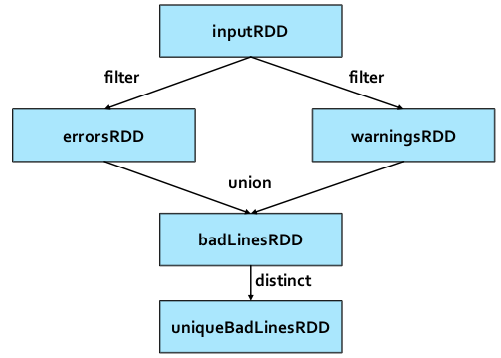
\includegraphics[width=4cm,height=4cm]{./img/data.png}
\caption{\label{fig:orgbba4f22}DAG corresponding to the listing}
\end{figure}
\end{column}
\end{columns}
\end{frame}

\section{Dockerize your environment}
\label{sec:orga76c973}

\begin{frame}[label={sec:orgcf98488},fragile]{Requirements}
 \begin{itemize}
\item A working Docker environment on your machine -- if your are on Fedora (>==32), you should 
use \texttt{podman} instead of Docker
\item You should be familiar with the notions of:
\begin{itemize}
\item Docker image
\item Docker container
\item Dockerfile
\end{itemize}
\end{itemize}
\end{frame}

\begin{frame}[label={sec:orgcc58f31}]{Dockerize your environment}
\begin{itemize}
\item The following Dockerfile creates a working environment with everything you need: Scala, sbt and Spark
\end{itemize}

\begin{columns}
\begin{column}{0.5\columnwidth}
\begin{figure}[htbp]
\centering
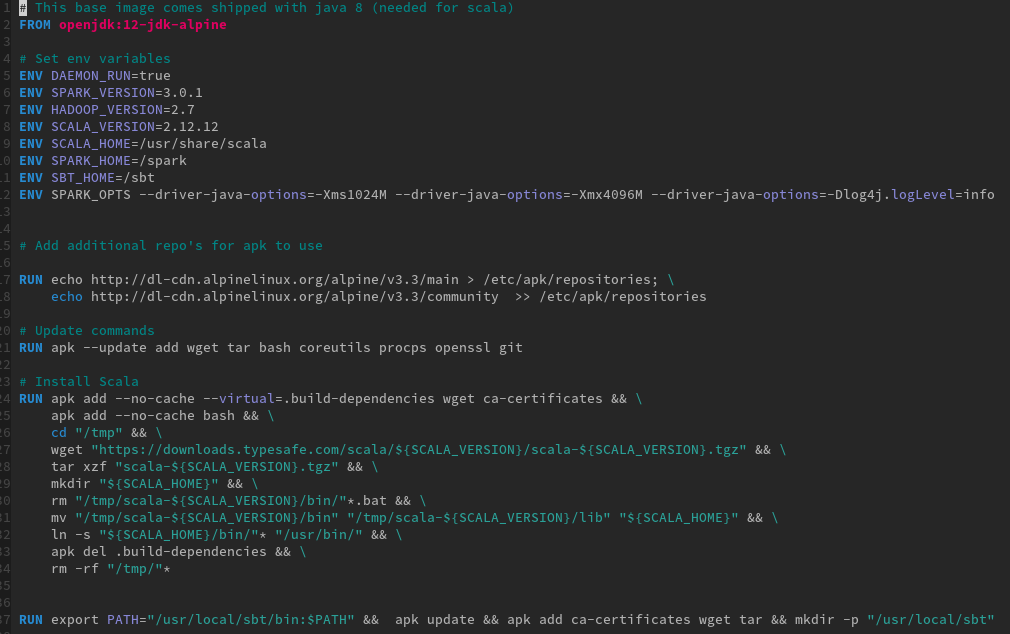
\includegraphics[width=7cm,height=4cm]{./img/dockerfile1.png}
\caption{\label{fig:org680d391}First part}
\end{figure}
\end{column}


\begin{column}{0.5\columnwidth}
\begin{figure}[htbp]
\centering
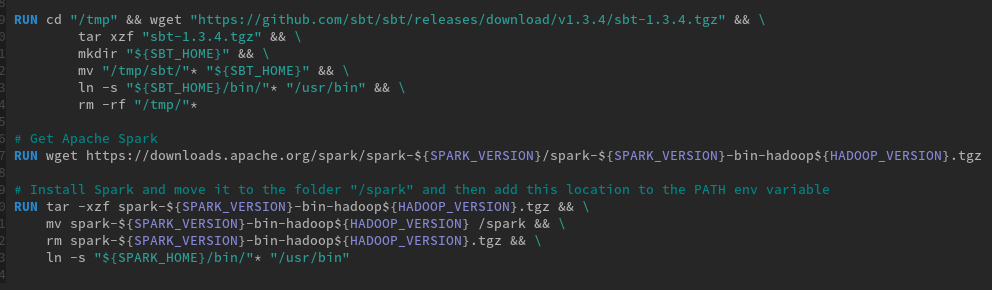
\includegraphics[width=7cm,height=2cm]{./img/dockerfile2.png}
\caption{\label{fig:org42626b2}Second part}
\end{figure}
\end{column}
\end{columns}
\end{frame}


\begin{frame}[label={sec:orga86dab0},fragile]{Dockerize your application}
 \begin{itemize}
\item A very simple way to  dockerize your application is to put the following file
inside the root directory of your project
\end{itemize}
\begin{verbatim}
FROM <your-repository>/spark-base

RUN mkdir /app
COPY . /app
WORKDIR /app # this is the working directory inside your container

\end{verbatim}
\begin{itemize}
\item Then within the same directory you build the container as follows:
\end{itemize}
\begin{verbatim}
docker image build -t <imageName> .
\end{verbatim}
\begin{itemize}
\item Finally, you run the container as follows:
\end{itemize}
\begin{verbatim}
docker run --rm -it -v $(pwd):/app <imageName> spark-submit --class <MainClass> ... 
\end{verbatim}
\end{frame}
\end{document}